% Asset ID: AS1GraphsTransformationsTikZ-002
% Source: DrFrost Chapter 4 repeated-root examples and transcript
% Purpose: Compare simple, repeated and triple repeated roots
\documentclass[tikz,border=8pt]{standalone}
\usepackage{pgfplots}
\pgfplotsset{compat=1.18}
\begin{document}
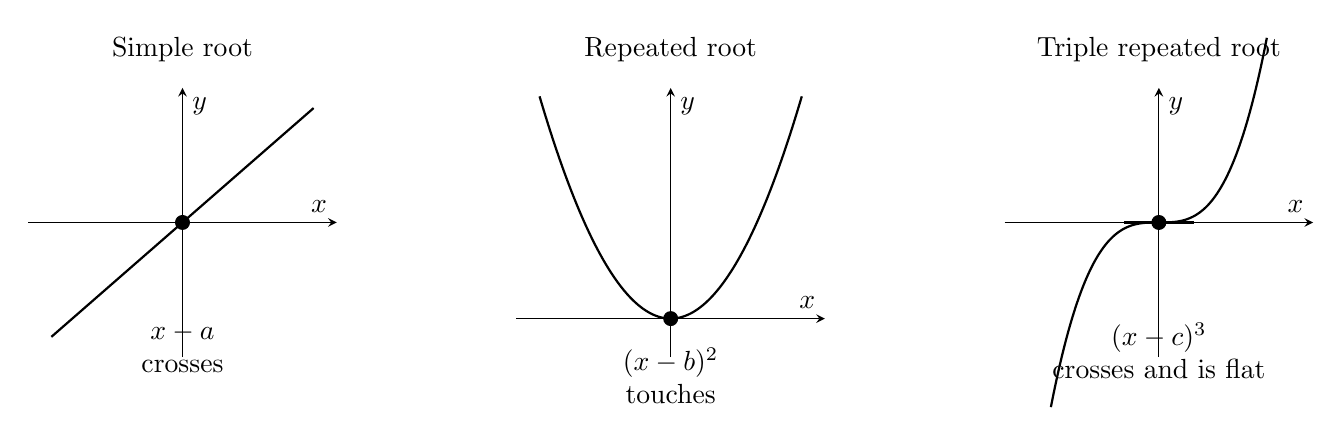
\begin{tikzpicture}
\begin{axis}[name=simple,at={(0,0)},anchor=south west,axis lines=middle,xmin=-2,xmax=2,ymin=-2,ymax=2,width=5.5cm,height=5cm,xtick={0},xticklabels={$a$},ytick=\empty,xlabel={$x$},ylabel={$y$},title={Simple root},samples=100,domain=-1.7:1.7,grid=both,clip=false]\addplot[thick]{x};\addplot[only marks,mark=*,mark size=2.5pt] coordinates{(0,0)};\node[align=center,anchor=north] at (axis cs:0,-1.35){$x-a$\\crosses};\end{axis}
\begin{axis}[name=repeated,at={(6.2cm,0)},anchor=south west,axis lines=middle,xmin=-2,xmax=2,ymin=-0.5,ymax=3,width=5.5cm,height=5cm,xtick={0},xticklabels={$b$},ytick=\empty,xlabel={$x$},ylabel={$y$},title={Repeated root},samples=100,domain=-1.7:1.7,grid=both,clip=false]\addplot[thick]{x^2};\addplot[only marks,mark=*,mark size=2.5pt] coordinates{(0,0)};\node[align=center,anchor=north] at (axis cs:0,-0.25){$(x-b)^2$\\touches};\end{axis}
\begin{axis}[name=triple,at={(12.4cm,0)},anchor=south west,axis lines=middle,xmin=-2,xmax=2,ymin=-2,ymax=2,width=5.5cm,height=5cm,xtick={0},xticklabels={$c$},ytick=\empty,xlabel={$x$},ylabel={$y$},title={Triple repeated root},samples=100,domain=-1.4:1.4,grid=both,clip=false]\addplot[thick]{x^3};\addplot[only marks,mark=*,mark size=2.5pt] coordinates{(0,0)};\draw[thick](axis cs:-0.45,0)--(axis cs:0.45,0);\node[align=center,anchor=north] at (axis cs:0,-1.35){$(x-c)^3$\\crosses and is flat};\end{axis}
\end{tikzpicture}
\end{document}
